\documentclass[a4paper,openany,12pt]{book}
\usepackage{graphicx}
\usepackage[utf8]{inputenc}

\usepackage[spanish]{babel}
\usepackage{fancyhdr}
\usepackage{ae}
\usepackage[left=2.5cm,right=2.5cm,top=3cm,bottom=2cm]{geometry}
\usepackage[printonlyused]{acronym}
\usepackage{xspace}
\usepackage{hlundef}
\usepackage{tesis}
\usepackage{setspace}

\title{Título de la Tesis}

\author{Nombre del Alumno}

\advisor{Prof Dr./Mag./Ing. Nombre del Asesor}

\examinerone{Prof. Dr. Hidalgo Buena Gente}{Presidente}%
\examinertwo{Prof. Dr. Manuel Armando Líos}{Secretario}%
\examinerthree{Prof. Dr. Antero A. Gal Oppe}{Integrante}%
\examinerfour{Prof. Dr. Casso E. Staria}{Externo}{Universidad del ABC} % of being the case
\date{30 de Junio del 2004}
\date{\today}

\dedicado{Aquí deberás colocar a quien va dedicada tu tesis por ejemplo: A Dios, por todo lo que me ha dado, a todos los profesores por sus enseñanzas y algunos amigos.}

\begin{document}
\pagestyle{fancy}

\maketitle %Compone la carátula y la dedicatoria
\newpage

\approved{\cuatro}%  {\tres} or {\cuatro}

%mayores detalles de como usas las abreviaturas (acronimos)
% vea: http://www.ctan.org/tex-archive/macros/latex/contrib/acronym/
% hay un manual en pdf en esa misma direccion

\chapter*{Abreviaturas}

\begin{acronym}
\acro{SPC}{Sociedad Peruana de Computación}
\acro{CMM}{\textit{Capability Maturity Model}}
\end{acronym}


\begin{agradecimientos}
Aquí deberás colocar a quien y porque agradeces. Ejemplo:

En primer lugar deseo agradecer a Dios por haberme guiado a lo largo de estos cinco años de estudio.

Agradezco a mis padres por el apoyo brindado para forjarme como un profesional.

Agradezco a la universidad, mi \textit{alma matter}, por haberme cobijado y brindado la formación que ahora me permitirá ayudar a construir una mejor sociedad.

Agradezco de forma muy especial a mi orientador Prof. Dr./Mag. nombre 1 por haberme guiado en esta tesis. ...

Deseo agradecer de forma especial a mis docentes: nombre 1, nombre 2, nombre 3 porque fueron ejemplos que deseo seguir en mi vida profesional.

Deseo agradecer al personal administrativo de la universidad: nombre 1, nombre 2, nombre 3. Muchas gracias por la atención brindada y porque siempre estuvieron dispuestas a ayudarnos.
\end{agradecimientos}
 %Inserta los agradecimientos
\begin{resumen}

El desarrollo de videojuegos, especialmente del género RPG, supone el uso en conjunto de una serie de tópicos que llevan al límite los recursos disponibles para la consolidación del mismo. El diseño de argumentos y la generación de eventos en torno a este suponen una tarea sumamente importante pues tendrán un gran efecto en la experiencia del jugador. Debido a esto la construcción de un guión (o guiones) es una tarea en la cual se hace necesario invertir una gran cantidad de esfuerzo. Bajo esta premisa, se propone un sistema capaz de automatizar estas tareas al generar eventos relacionados a una historia central utilizando al mismo tiempo modelos de personalidad que permitan distinguir las preferencias del jugador. La aplicación de este sistema permitiría reducir los recursos destinados al diseño de un argumento aligerando a la vez la carga tras el desarrollo de un videojuego.


\end{resumen}
 %Inserta el resumen
\begin{abstract}
Here you must write between 100 and 150 words about your thesis. 

In this text you must highlight your main contributions to this field.
\end{abstract}
 %Inserta el abstract

\pagenumbering{roman}
\setcounter{page}{1}
\pagestyle{plain}

\tableofcontents %Inserta el índice general
\listoftables %Inserta el índice de cuadros
\listoffigures %Inserta el índice de figuras

%%%%%%%%%%%%%%%%%%%%%%%%%%%%%%%%%%%%%%%%%%%%%%%%%%%%%%%%%%%%%%%%%%%%%
%%%%   En esta parte deberas incluir los archivos de tu tesis   %%%%%
%%%%%%%%%%%%%%%%%%%%%%%%%%%%%%%%%%%%%%%%%%%%%%%%%%%%%%%%%%%%%%%%%%%%%

\pagestyle{plain}
\pagenumbering{arabic}
\setcounter{page}{1}
\chapter{Introducción}

%Este es el primer capítulo de la tesis. Se inicia con el desarrollo de la introducción de la tesis. Es importante que el texto utilice la tabla de abreviaturas correctamente. En el archivo abreviaturas.tex contiene la tabla de abreviaturas. Para citar alguna de ellas debes usar los comandos $\backslash$ac\{tu-sigla-aqui\}. Si es la primera vez que utilizas la sigla ella se expandirá por completo. Por ejemplo, el comando $\backslash$ac\{CMM\} va a producir: \ac{CMM}. Si más adelante repites el mismo comando sólo aparecerá la sigla \ac{CMM}. Para explorar mucho más este comando es necesario leer su manual disponible en: $http://www.ctan.org/tex-archive/macros/latex/contrib/acronym/$


\section{Motivación y Contexto}

%En esta sección se va desde aspectos generales a  aspectos específicos (como un embudo). No se olvide que es la primera parte que tiene contacto con el lector y que hará que este se interese en el tema a investigar. El objetivo de esta sección es llevar al lector hacie el tema que se va a tratar en forma específica y dejar la puerta abierta a otras investigaciones

Con la acelerada expansión del mundo de los videojuegos y su cada vez mayor influencia en la vida de sus jugadores, se hace necesario comprender que factores son súmamente influyentes en el éxito de una franquicia. Dentro del género \ac{RPG}, videojuegos tales como: \textit{The Elder Scrolls: Skyrim}, \textit{Fallout 3}, \textit{The Witcher}, \textit{Dying Light}, etc han llegado a alcanzar estatus de culto debido al impecable manejo de cuatro pilares fundamentales: Mecánicas, Estética, Tecnología e Historia \cite{schell2019art}. 

Si bien no existe un concepto más importante que otro (al menos durante la etapa de desarrollo), destacaremos el ámbito de la historia al ser uno de los más influyentes en la experiencia del jugador y por ser además el enfoque principal de esta investigación. Contar historias no es una tarea fácil. Al crear y narrar una histora se hace uso de la Inteligencia Narrativa. El propósito de esta es trasmitir una experiencia formada a partir de sucesos reales o ficticios. Dentro del mundo de los videojuegos, las historias representan el eje central en torno al cual giran las experiencias propias del jugador (especialmente en videojuegos del género \ac{RPG}). Una historia puede a la vez ser dividida en pequeños fragmentos que separados conforman los \textit{quests}(misiones) \cite{doran2010towards} que el jugador tendrá superar para llegar a la completitud de la historia principal. Estos \textit{quests} son también el punto principal de partida para argumentos secundarios que pueden llegar a alargar un poco más la vida útil de un videojuego. 

A pesar de su importancia, la aplicación de \textit{quests} en un videojuego conlleva a la realización de una tarea titánica. Enfocados ya en el género \ac{RPG}, es normal que la mayoría de \textit{quests} a resolverse (ya sean principales o secundarios) hayan sido desarrollados bajo la estricta supervisión de un escritor o guionista \cite{cheong2016planning}. Esto por lo general es lo más adecuado. Actualmente no se dispone de sistemas capaces de crear una historia desde cero, por lo que la participación humana se vuelve necesaria y justificable. Sin embargo, el problema principal no radica en las historias en sí, sino en la cantidad de historias que deben desarrollarse. Juegos como \textit{The Elder Scrolls: Skyrim}, \textit{Dying Light} o \textit{Final Fantasy} se caracterizan por poseer una cantidad muy alta de \textit{quests} secundarios en donde cada subargumento ha sido cuidadosamente planteado y desenvuelto. El esfuerzo puesto para que cada pequeña historia haya sido traducida hacia un contexto de \textit{quests} se traduce en varios días de desarrollo y aún así el resultado final es estático e invariable pues definido el \textit{quest}, la serie de eventos que lo conforman es inalterable, por lo que la experiencia del jugador es invariable. 

Para la solución de esta problemática proponemos el sistema CARDINAL. CARDINAL es un sistema diseñado para reconocer el modelo de personalidad que caracteriza a un jugador mediante el uso de una red neuronal y un \textit{test} de personalidad conocido como \textit{The Big Five}. El modelo conformado por cinco parámetros: Extraversión, Apertura a la experiencia, Responsabilidad, Amabilidad y Estabilidad Emocional se obtiene al inicio del juego mediante el uso de 10 escenas introductorias  y se modifica de forma periódica conforme el jugador va desénvolviendose en las mecánicas imbuidas del juego.  Definido el modelo de personalidad, CARDINAL procede a utilizar el Módulo de Planeamiento compuesto por dos submódulos secundarios: El submódulo de Historia y el submódulo de Discurso. En el submódulo de Historia se obtiene la secuencia de eventos que conforman un \textit{quest}. Este submódulo utiliza un planeador \ac{HTN} y para su funcionamiento se hace necesario la definición de un estado inicial (descripción del mundo al inicio del juego). Por otra parte, el submódulo de Discurso es el encargado de desenvolver la historia de una forma tal que resulte atractiva para el jugador (ya sea alterando las mecánicas del juego o modificando la secuencia de eventos en un \textit{quest}). Ambos submódulos trabajan de forma conjunta con el Modelo de Personalidad  siendo para el submódulo de Historia un parámetro útil para definir el tipo de \textit{quest} (Lugar, Tiempo u Objetivo) y para el submódulo de Discurso una variable que describe el estilo de juego en el jugador. Finalmente, y tras haber definido un plan de acción para el jugador, CARDINAL utiliza un módulo de control que verifica que los planes creados por el submódulo de Historia lleguen a concretarse y en caso sea necesario los elimine cuando las condiciones de desarrollo hacen que sea imposible concretar un plan (Condiciones como estas se dan cuando dos planes se interceptan y uno destruye las variables de desenvolvimiento del otro.)

Si CARDINAL llega concretarse, el desarrollo de \textit{quests} que describan segmentos de la historia podría automatizarse a tal grado que la participación de el escritor sería solo necesaria para definir un marco general de acciones en el mundo (estado inicial del juego). La aplicación de este sistema permitiría además obtener un desenvolvimiento de \textit{quests} dinámico en donde los patrones de comportamiento del jugador modifiquen las mecánicas del juego haciendo de la experiencia una novedad frente al desenvolvimiento estático de los \textit{quests} en los \ac{RPG} tradicionales.
 

\section{Planteamiento del Problema}

En el paradigma tradicional de desarrollo de videojuegos RPG, convertir una historia en un conjunto de \textit{quests} es una tarea extensa y laboriosa. Además, los resultados de este enfoque suelen ser  bastante estáticos e invariables debido al alto grado de autoría que poseen. Estas dos desventajas se traducen en un esfuerzo de desarrollo excesivo y en un videojuego limitado a las opciones argumentales que le han sido programdas. 


\section{Objetivos}

%1En esta sección se colocan los objetivos generales de la tesis. Máximo dos. Si necesita ampliar estos objetivos utilice la sección de objetivos específicos.
%Cardinal es una propuesta centrada en aligerar la carga tras los diseños argumentales de un videojuego. Esto no implica prescindir de un guionista o escritor, sino más bien reducir el esfuerzo autorial que este realizaría al desarrollar enteramente un argumento.

Implementar CARDINAL, un sistema enfocado en aligerar la carga tras los diseños argumentales de un videojuego. Esto no implica prescindir de un guionista o escritor, sino más bien, reducir el esfuerzo autorial que este realizaría dándole al sistema la opción de desarrollar una historia acorde a los gustos pasivos del jugador.


\subsection{Objetivos Específicos}

\begin{itemize}
\item Implementar un módulo para el reconocimiento de la personalidad mediante el uso de una red neuronal y un test de personalidad conocido como \textit{The Big Five}.

\item Implementar un módulo para la generación de planes utilizando un planeador \ac{HTN}, y tomando al modelo de personalidad como referencia para definir el tipo de \textit{quest} más adecuado para el jugador.

\item Implementar un módulo para el desenvolvimiento de un plan tomando también al modelo de personalidad como referencia. Este módulo será capaz de alterar la secuencia de eventos y modificar las mecánicas del juego acorde a un modelo de comportamiento imbuido en el modelo de personalidad del jugador.  

\item Implementar un módulo de control en donde los planes generados por el módulo de Historias sean verificados de manera constante. En caso sea necesario, este módulo tendrá la capacidad de  eliminar los planes que resulten imposiles de concretar. 

  
\end{itemize}


\section{Cronograma}

\begin{table}[]
\caption{Tabla de Actividades}
\label{tab:tab4}
\begin{tabular}{|l|l|l|l|}
\hline
\multicolumn{1}{|c|}{Desde}      & \multicolumn{2}{c|}{Hasta}      & Actividad                                                                                                                                                       \\ \hline
\multicolumn{1}{|c|}{03/09/2019} & \multicolumn{2}{c|}{01/10/2019} & Redacción del Plan de Tesis                                                                                                                                     \\ \hline
\multicolumn{1}{|c|}{06/09/2019} & \multicolumn{2}{c|}{10/09/2019} & \begin{tabular}[c]{@{}l@{}}Redacción del Capítulo 1 (Introducción): Objetivo General, \\ Objetivos Específicos, Motivación Contexto, Planeamiento.\end{tabular} \\ \hline
\multicolumn{1}{|c|}{10/09/2019} & \multicolumn{2}{c|}{12/09/2019} & Corrección del Capítulo 1                                                                                                                                       \\ \hline
\multicolumn{1}{|c|}{13/09/2019} & \multicolumn{2}{c|}{13/09/2019} & Presentación del Capítulo 1                                                                                                                                     \\ \hline
\multicolumn{1}{|c|}{15/09/2019} & \multicolumn{2}{c|}{18/09/2019} & \begin{tabular}[c]{@{}l@{}}Redacción del Capítulo 2: \\ Estado del Arte, Marco Teórico\end{tabular}                                                             \\ \hline
\multicolumn{1}{|c|}{19/09/2019} & \multicolumn{2}{c|}{19/09/2019} & \begin{tabular}[c]{@{}l@{}}Revisión del Capítulo 2: \\ Estado del Arte, Marco Teórico\end{tabular}                                                              \\ \hline
20/09/2019                       & \multicolumn{2}{l|}{20/09/2019} & \begin{tabular}[c]{@{}l@{}}Presentación del Capítulo 2 \\ Estado del Arte / Marco Teórico\end{tabular}                                                          \\ \hline
20/09/2019                       & \multicolumn{2}{l|}{01/10/2019} & Finalización en la Redacción del Plan de Tesis                                                                                                                  \\ \hline
02/10/2019                       & \multicolumn{2}{l|}{06/10/2019} & \begin{tabular}[c]{@{}l@{}}Corrección de observaciones \\ encontradas en el Plan de Tesis.\end{tabular}                                                         \\ \hline
18/10/2019                       & \multicolumn{2}{l|}{18/10/2019} & Presentación y Aprobación del Plan de Tesis                                                                                                                     \\ \hline
20/10/2019                       & \multicolumn{2}{l|}{25/10/2019} & \begin{tabular}[c]{@{}l@{}}Implementación del modelo de personalidad \\ utilizando The Big Five. (5\% de resultados)\end{tabular}                               \\ \hline
26/10/2019                       & \multicolumn{2}{l|}{01/11/2019} & \begin{tabular}[c]{@{}l@{}}Implementación del Sistema para la \\ generación de quest utilizando CONAN (15\%)\end{tabular}                                       \\ \hline
02/11/2019                       & \multicolumn{2}{l|}{15/11/2019} & \begin{tabular}[c]{@{}l@{}}Implementación del Sistema para la generación \\ de quest utilizando StoryAssembler (35\%)\end{tabular}                              \\ \hline
16/11/2019                       & \multicolumn{2}{l|}{19/11/2019} & Redacción del Capítulo Resultados.                                                                                                                              \\ \hline
19/11/2019                       & \multicolumn{2}{l|}{20/11/2019} & Revisión del Capítulo Resultados.                                                                                                                               \\ \hline
21/11/2019                       & \multicolumn{2}{l|}{21/11/2019} & Presentación del Capítulo Resultados                                                                                                                            \\ \hline
24/11/2019                       & \multicolumn{2}{l|}{30/11/2019} & Redacción del Documento Avances de Tesis                                                                                                                        \\ \hline
01/12/2019                       & \multicolumn{2}{l|}{10/12/2019} & Presentación del Documento Avances de Tesis                                                                                                                     \\ \hline
\end{tabular}
\end{table}

 %Inserta el capítulo 1
\chapter{Trabajos Relacionados}

%Cada capítulo deberá contener una breve introducción que describe en forma rápida el contenido del mismo. En este capítulo va el marco teórico y el estado del arte. (pueden hacer dos capítulos: uno marco teórico y otro de estado del arte)


\section{Marco Teórico}

\ac{PCG-G} centrada en la generación narrativa puede describirse como un área enfocada en la producción de contenido argumental para el marco narrativo de un videojuego. Los enfoques tradicionalmente identificados son: Sistemas basados en Simulación y Sistemas Deliberativos \cite{garbe2019storyassembler}.

Los Sistemas basados en Simulación tienen por característica principal implementar una serie de reglas que rigen al mundo y a los personajes. Estas reglas actúan como una serie de condicionales que reflejan la intención principal de la historia y son en gran medida establecidas por el propio guionista de la historia. Estas restricciones en conjunto con todas las posibles acciones a realizar sirven de base para una generación sistemática de argumentos narrativos secundarios. Debido a esto, este enfoque suele ser considerado levemente caótico.

Por otro lado, los Sistemas Deliberativos comparten las mismas bases que el enfoque previo, más sin embargo, se diferencian por establecer situaciones a ser resueltas. Este plantemiento permite definir estados deseados a los cuales el sistema debe llegar con prioridad. Un sistema basado en este enfoque es \textit{StoryAssembler} \cite{garbe2019storyassembler}, el cual utiliza una librería de contenidos en donde se especifican las limitantes que posee cada fragmento y que posteriormente son presentadas al jugador a través de una narrativa basada en elecciones. 

Con las definiciones previas es posible definir el desenvolvimiento de un \textit{quest}. Los \textit{quests} son por lo general tareas encargadas por los personajes \ac{NPC} de un juego. Consisten en un grupo de acciones que deben realizarse en un orden en específico para poder alcanzar un objetivo (la mayoría de veces una recompensa) \cite{breault2018let}. Los \textit{quests} representan una parte del contenido narrativo por lo que su desenvolvimiento debe ir acorde con el estado del mundo y la actitud de los \ac{NPC}. Bajo este marco, un \textit{quest} derivado de la aplicación de un sistema \ac{PCG-G} implica el uso de un Agente Inteligente de Planeamiento. Debido a la similitud estructural entre los resultados de estos agentes y el contenido de un \textit{quest}, es posible implementar sistemas como \cite{doran2011prototype} \cite{riedl2011game} \cite{yu2012sequential} en donde historias creadas por humanos son modificadas por IAs de planeamiento siguiendo una serie estados en donde se definen el inicio y el orden de eventos. También es importante destacar que en el orden se debe considerar con prioridad un correcto progreso Lógico-Causal que refleje que los eventos ocurridos a lo largo de la historia obedecen a reglas que favorecen la \textbf{credibilidad del personaje}(percepción por parte del jugador en  donde un personaje actúa de manera coherente).

Enfocado el tema de \textit{quests} podemos clasificarlos en tres categorías segun \cite{cheong2016planning}

\begin{itemize}
\item[•] \textit{Place Oriented Quests} son aquellos en donde el jugador debe de moverse por el mundo hacia un lugar especificado y con ciertas pruebas a lo largo del camino.
\item[•] \textit{Time Oriented Quests} son aquellos considerados como pruebas de resistencia en donde el jugador debe sobrevivir durante un determinado periodo de tiempo.
\item[•] \textit{Objective Oriented Quests} son aquellos caracterizados por la necesidad de cumplir un objetivo (Conseguir un objeto, traer un aliado, eliminar un enemigo, etc.)
\end{itemize}

Todas estas categorías pueden mezclarse de manera tal que mientras se respete el marco narrativo, hagan más atractiva la experiencia del jugador.

Cuando los \textit{quests} queden sujetos a definición por un Agente Inteligente de Planeamiento (A partir de ahora un Planificador), se debe considerar que tanto para un Sistema basado en Simulación como un Sistema Deliberativo, dicho Planificador deberá poseer un conocimiento total sobre todos los posibles eventos que pueden llegar a suceder. Esto incluye la definición de el Estado Inicial (descripción inicial del mundo) así como la definición de el Estado Objetivo (hacia donde debe llegar el Planificador). El objetivo de Planificador es encontrar una solución entre ambos estados, siendo la solución al problema de planeamiento un \textit{Plan} que contenga toda una secuencia de acciones. Cuando el Planificador es capaz de encontrar una solución entre el estado inicial y el estado objetivo, el resultado se conoce como \textit{Sound Plan} \cite{cheong2016planning}.

Por otra parte, el conjunto de eventos que maneja un Planificador se almacena como una librería de sucesos que toman el nombre de \textit{Operadores de Planeamiento} en donde cada operador está compuesto por un conjunto de \textit{Precondiciones} y un conjunto de \textit{Efectos}. Las Precondiciones representan las condiciones que deben alcanzarse para ejecutar el Operador mientras que los Efectos con condiciones que se vieron actualizadas tras el uso del Operador. Las soluciones obtenidas con la aplicación de estos operadores pueden representarse de dos maneras: 

\begin{itemize}

\item \textbf{Soluciones en el Espacio de Estados: } Es una representación en donde las soluciones son estructuradas en un árbol compuesto por nodos y arcos. En esta representación cada nodo es un estado y cada arco es la transición de un estado a otro tras la aplicación de un Operador. Si partimos del nodo raíz, este representará el Estado Inicial del mundo mientras que si nos dirigimos a este, este pasará a ser el Estado Objetivo

\item \textbf{Soluciones en el Espacio de Planes: }  Similar a la representación previa, en esta representación el árbol se vale solo de los nodos para figurar cada solución.  El nodo raíz almacena el problema de planeamiento, el Estado Inicial y el Estado Objetivo. Si no existe una solución directa entre ambos estados, el árbol proyecta un nodo hijo de la raíz en donde se añade un paso más para alcanzar la solución. Si este nodo hijo no alcanza la solución, este proyecta un nuevo nodo hasta que la solución se satisfaga. En esta representación, las hojas del árbol son soluciones completas o soluciones vacías.

\begin{figure}[tph!]
\centerline{
\includegraphics[totalheight=7cm]{3}}
    \caption{Grafo con Soluciones en el Espacio de Planes. \cite{cheong2016planning}}
    \label{fig:ptest1}
\end{figure}


\end{itemize}

\subsection{Planning Story}

La representación de una historia derivada del uso de un Planificador puede definirse como una Tupla: $<S, O, C>$ en donde :

\begin{itemize}
\item S es un conjunto de eventos procedente de la librería de Operadores.
\item O representa el orden temporal entre dos eventos $S_1, S_2$, en donde $S_1$ precede a $S_2$.
\item C es una lista de representa la causalidad entre $(s, t, c )$ en donde $s$ pasará a $c$ al cumplir la precondición $t$

\end{itemize}

\section{Estado del Arte}

Si bien existen múltiples técnicas para Agentes Inteligentes de Planeamiento, muy pocas de ellas han sido orientadas a su aplicación directa en videojuegos. La mayoría de técnicas que describiremos a continuación vieron su aplicabilidad en la formulación de historias a partir de elecciones hechas por el usuario y no por eventos sugestionados por el mismo sistema.

\subsection{Story Assembler}

Story Assembler \cite{garbe2019storyassembler} es un sistema orientado a la Narrativas Basadas en Elecciones. Es un excelente ejemplo en el marco de \textit{StoryTelling} puesto que presenta un alto grado de interactividad con el usuario. La característica principal de \textit{Story Assembler} es que forma parte de la familia de sistemas centrados en la Hiperficción (Un análogo de los libros \textit{Escoge tu propia aventura}) y al mismo tiempo posee características de Sistemas Manejados por Planeamiento. Esta naturaleza dual permite que Story Assembler no dependa de mucho contenido autorial pues el ensamblaje de nuevas historias es un proceso enteramente computacional.

\begin{figure}[tph!]
\centerline{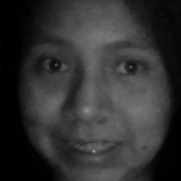
\includegraphics[totalheight=7cm]{1}}
    \caption{Planificador \textit{Story Assembler} y relación con fragmentos de textos. \cite{garbe2019storyassembler}}
    \label{fig:ptest1}
\end{figure}


\textit{Story Assembler} es un Sistema Deliberativo en donde se establecen los estados prioritarios que el sistema debe alcanzar. Funciona de manera  muy similar a un planificador \ac{HTN} pues crea eventos a partir de una librería de fragmentos de texto utilizando párrafos de textos más grandes. Cuando es ejecutado, \textit{Story Assembler} revisa las variables del estado inicial y las variables del estado deseado para posteriormente proceder a ensamblar fragmentos que lo acerquen cada vez más a su objetivo. Si el sistema ubica fragmentos de texto que lo acerquen de manera significativa, este procederá a juntarlos y tratarlos como un fragmento de texto único. Al final de una iteracción, el mejor fragmento esamblado representará el siguiente paso que el sistema dé para alcanzar su estado objetivo. 

\subsection{Let CONAN tell you a story} 

CONAN \cite{breault2018let} es un sistema de generación procedural de \textit{quest} aplicados en videojuegos (Muy similar a CARDINAL). Como casi todos los planificadores, funciona a partir de un estado inicial y de un conjunto que defina todas las posibles acciones a realizar en el mundo. CONAN es un sistema de simulación, es decir que a diferencia del modelo previo, acá no existen estados deseables que el sistema deba alcanzar. De hecho, podríamos definir a CONAN como un conjunto de pequeños agentes inteligentes de planeamiento. Cuando el sistema es puesto en marcha, cada \ac{NPC} dentro del juego revisará los objetivos que posee e implementará un plan que le será comunicado al jugador como un \textit{quest}. Por ejemplo, si un panadero \ac{NPC} se quedase sin material para seguir fabricando pan, entonce el planificador tras este identificará el nuevo problema de  conseguir Harina como un \textit{quest} para el jugador.

Para cada planificador en CONAN se requiere de los siguientes elementos:

\begin{itemize}
\item \textbf{Estado Inicial:} Es un estado estándar que representa el punto de partida para cada uno los \ac{NPC} y para el mundo en general. Definir un estado inicial en CONAN significa enfocarse en aspectos tales como: Localizaciones, Descripciones e Interconexiones. Además, cada pequeño agente en este sistema estará provisto de un conjunto de preferencias definidos en relación a un peso descrito en sus acciones. 

\item \textbf{Documento de Dominio:} Contiene todas las posibles acciones que puede realizar un personaje para poder alcanzar un objetivo. Más allá de estos, uno no podrá recurrir a acciones que lo fueron designadas.

\item \textbf{Generación de Objetivos: } Para cada planificador individual un objetivo es un estado que deber verdadero en el mundo solamente para el. En CONAN la definición de un objetivo puede realizarse de dos formas: Aleatoriamente y Aleatoriamente pero considerando las prioridades de cada planificador. 

\end{itemize}

\begin{figure}[tph!]
\centerline{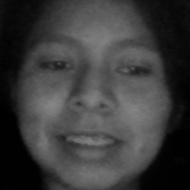
\includegraphics[totalheight=7cm]{2}}
    \caption{Desenvolvimiento del planificador \textit{CONAN}. \cite{breault2018let}}
    \label{fig:ptest1}
\end{figure}

\subsection{Story and Discourse}

Más que un sistema para la generación procedural de \textit{quests}, \textit{Story and Discourse} \cite{young2007story} es un modelo centrado en representar los dos aspectos básicos de la narrativa dentro de los mundos virtuales: Historia y Discurso. 

La historia se define como la serie de eventos por los que el personaje principal ha de pasar. Esta incluye además el planificador que se utilize (Para \textit{Story and Discourse} fue un planificador \ac{DPOCL}), algunos aspectos prácticos de la narratología como el suspenso, la originalidad o el interés y el porque se carece de modelos capaces de generar historias desde cero. 

Por otro lado, el discurso es el aspecto más práctico de la narratología. En este concepto se incluyen todas las formas que existen para transmitir una historia al jugador. Por ejemplo, si la historia de un videojuego señala el enfrentamiento entre antagonista y protagonista, el discurso de dicha historia sería cada fotograma que refleje dicho enfrentamiento. 
























%\section{Sección 1 del Capítulo II}

%Un capítulo puede contener n secciones. La referencia bibliográfica se hace de la siguiente manera: \cite{Mateos00}

%\subsection{Sub Sección}

%Una sección puede contener n sub secciones.\cite{Galante01}


%\section{Recomendaciones generales de escritura}
%Un trabajo de esta naturaleza debe tener en consideración varios aspectos generales:

%\begin{itemize}
%\item Ir de lo genérico a lo específico. Siempre hay qeu considerar que el lector podría ser alguien no muy familiar con el tema y la lectura debe serle atractiva.
%\item No poner frases muy largas. Si las frases son de mas de 2 líneas continuas es probable que la lectura sea dificultosa.
%\item Las figuras, ecuaciones, tablas deben ser citados y explicados {\bf antes} de que aparezcan en el documento.
%\item Encadenar las ideas. Ninguna frase debe estar suelta. Siempre que terminas un párrafo y hay otro a continuación,  el primero debe dejar abierta la idea que se explicará a continuación. Todo debe tener secuencia.
%\end{itemize}
 %Inserta el capítulo 2
\chapter{CARDINAL}

%En este capítulo se desarrolla toda la propuesta realizada a través de la investigación. Sigue la misma estructura del capítulo anterior.
%El título del capítulo es flexible de acuerdo a cada tesis. Algunos títulos sugeridos podrían ser:
%Este título debe de estar ade acuerdo con el asesor del tema. Consúltelo en su sala de clase.

CARDINAL es un sistema de simulación con una propuesta enfocada en la utilización de tres pilares claves. 

El primer pilar implica la identificación de un modelo de personalidad-comportamiento que evolucione conforme el jugador va desenvolviéndose a lo largo del juego. Dicho modelo se obtiene mediante la aplicación de dos técnicas:
\begin{itemize}
\item \textit{The Big Five Test} es un cuestionario de 10 preguntas que permite identificar un modelo básico de la personalidad al establecer una serie de escenarios que al ser resueltos, definen los parámetros iniciales de Extraversión, Apertura a la experiencia, Responsabilidad, Amabilidad y Estabilidad Emocional

\item La segunda técnica es una propuesta hecha por \cite{de2018player}. Mediante el uso de una red neuronal entrenada bajo variables relacionadas a las mecánicas del juego, se hace posible la obtención de un modelo de comportamiento. De manera similar al modelo personalidad, el modelo de comportamiento también se define bajo los estándares de \textit{The Big Five} con la diferencia de que este modelo es dinámico, pues varía conforme el jugador se va desenvolviendo en el videojuego.
\end{itemize}

Finalmente, la obtención del modelo personalidad-comportamiento se obtiene de la ponderación de los modelos previos. Esta última etapa requiere de la aplicación de una variable de influencia que permita asignar el grado de perticipación que tiene cada modelo componente. En este caso, y debido a la naturaleza del videojuego en el que nos efocamos (RPG), se dará prioridad al modelo de personalidad. 

El segundo pilar fundamental se traduce en la implementación de un módulo de planeamiento. Este módulo basado en las propuestas hechas por \cite{young2007story} se divide en dos submódulos que cubren cada aspecto de la narratología en un videojuego:

\subsection{Submódulo de Historia}

Es un componente centrado en la creación de historias a partir de una planificador \ac{HTN}. Al igual que la propuesta hecha en \cite{breault2018let} cada personaje \ac{NPC} dentro del juego busca siempre alcanzar un objetivo que puede traducirse en un nuevo \textit{quest} para el jugador. Estos objetivos nuevos ingresan al planificador \ac{HTN} junto con el modelo de personalidad. El planificador pondera entonces cuáles son las inclinaciones del jugador en ese instante y procede con la creación de un quest basado en las siguientes consideraciones:

\begin{itemize}
\item Si el jugador posee un alto grado de extraversión se priorizará la generación de \textit{quests} con carácter de búsqueda.
\item Si el jugador posee un alto grado de apertura a la experiencia se priorizará la generación de \textit{quests} con carácter de exploración.
\item Si el jugador posee un alto grado de responsabilidad se priorizará la generación de \textit{quests} con carácter de resistencia.
\item Si el jugador posee un alto grado de amabilidad se priorizará la generación de \textit{quests} con carácter de búsqueda.
\item Si el jugador posee un alto grado de estabilidad emocional se priorizará la generación de \textit{quests} con carácter de resitencia.
\end{itemize}

Cabe recalcar que las definiciones previas son solo conceptos de carácter experimental por lo que su validez dependerá de como se desenvuelvan al momento de ser implementados.

\subsection{Submódulo de Discurso}

El submodulo de Discurso en CARDINAL no es equivalemente al concepto de Discurso en \cite{young2007story}. Discurso en un submódulo casual enfocado en dinamizar la mecánicas del juego en relación al modelo de comportamiento derivado del modelo personalidad del jugador. Considerando la propuesta hechas por \cite{de2018player}, se planea listar la misma serie de mecánicas para ofrecer el mismo comportamiento adaptativo. Si por ejemplo, la red neuronal detecta a un jugador actuando de manera muy violenta, el submódulo de discurso modificará la naturaleza de los enemigos haciéndolos más agresivos o más resitentes al daño. Por otro lado, si el jugador demuestra un carácter más precavido, se enfrentará a enemigos más astutos y a situaciones en donde la estrategia ira por sobre la fuerza bruta. 

Este submódulo posee además la capacidad de reestructurar la secuencia de eventos actuales (Esto no implica modificar la historia)\cite{de2018player}. Si por ejemplo el jugador tiene inclinacíón hacia la exploración y búsqueda de lugares ocultos, el submódulo se encargará de habilitar la mayor cantidad de lugares secretos. Caso contrario, si el jugador apenas demuestra interés por salirse de la ruta tradicional, el submódulo se centrará en mandar una mayor cantidad de enemigos y habrá menos recompensas por parte de los lugares ocultos.

El tercer y último pilar de CARDINAL es un módulo de control. Cada vez que el módulo de planeamiento genera una nueva historia, existe la posibilidad de que otras historias vean afectadas su desenvolvimiento. Este error por lo general se produce cuando los efectos de un Operador en el Planificador afectan la ejecución de otro Operador pues inválida sus precondiciones. En estos casos, concretar dicha misión se vuelve virtualmente imposible siendo necesaria su pronta eliminación. Otra labor que lleva a cabo el módulo de control es la de revisar de manera frecuente las precondiciones y los efectos de cada Operador  en la librería de eventos. Si se ubica una incoherencia, se hace necesario una corrección inmediata











 

















































 %Inserta el capítulo 3
\chapter{Pruebas y Resultados}
 %Inserta el capítulo 4
\chapter{Conclusiones}\label{chap:conclusiones}

Colocar Conclusiones  %Inserta el capítulo 5

%%%%%%%%%%%%%%%%%%%%%%%%%%%%%%%%%%%%%%%%%%%%%%%%%%%%%%%%%%%%%%%%%%%%%%

\bibliographystyle{apalike}
\bibliography{Bibliog}
\addcontentsline{toc}{chapter}{Bibliografía}
\end{document}
